\documentclass[PICOReport.tex]{subfiles}

\begin{document}

\begin{figure*}
%\vskip-3cm
\begin{center}
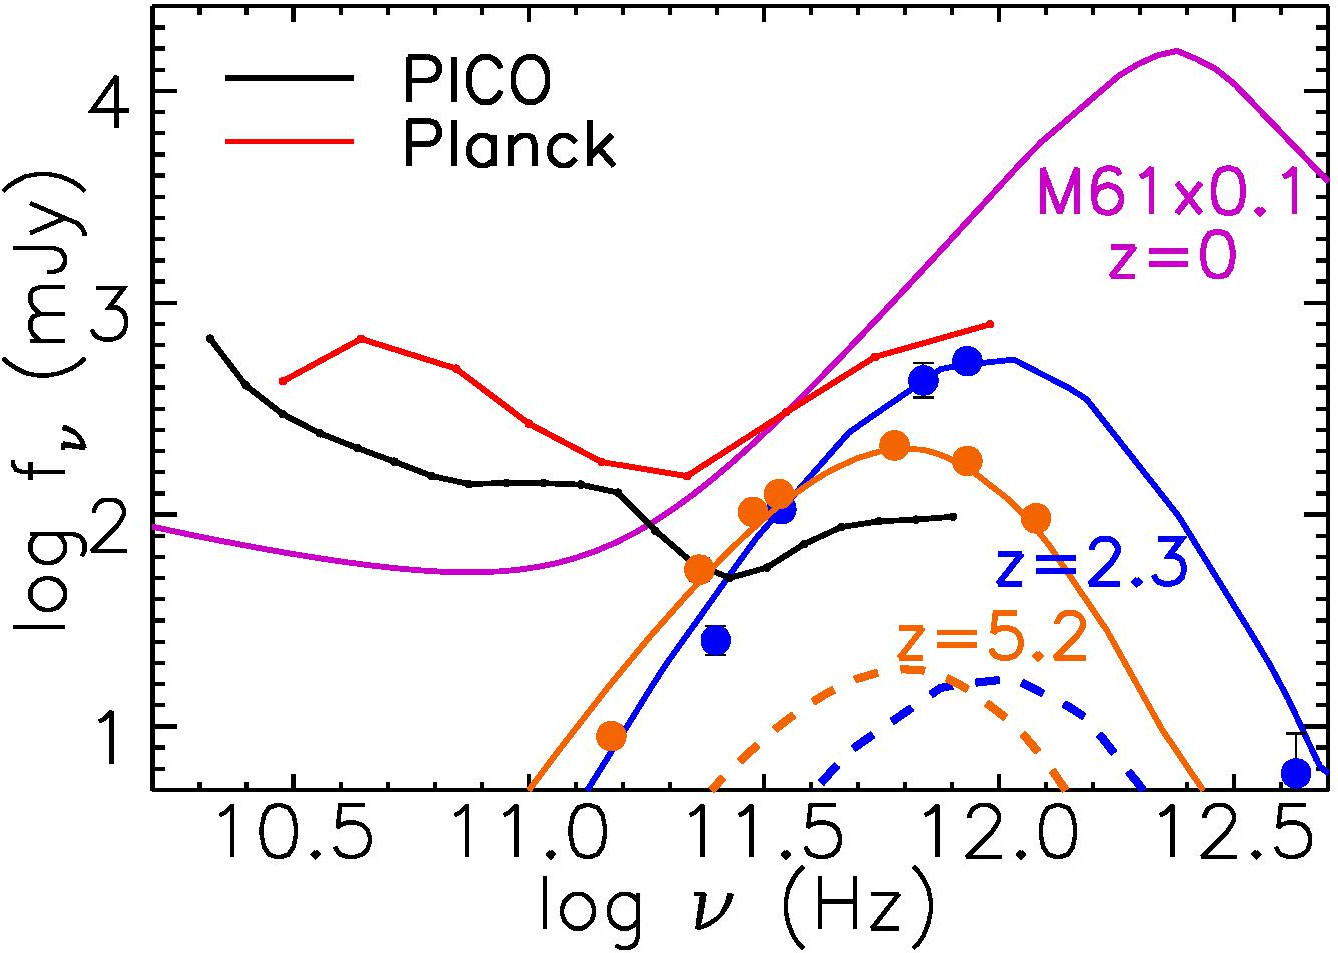
\includegraphics[width=0.41\columnwidth, trim={0 0 0 0cm}, clip]{images/fig_SED_PICO.jpg}
\hspace{0.75cm}
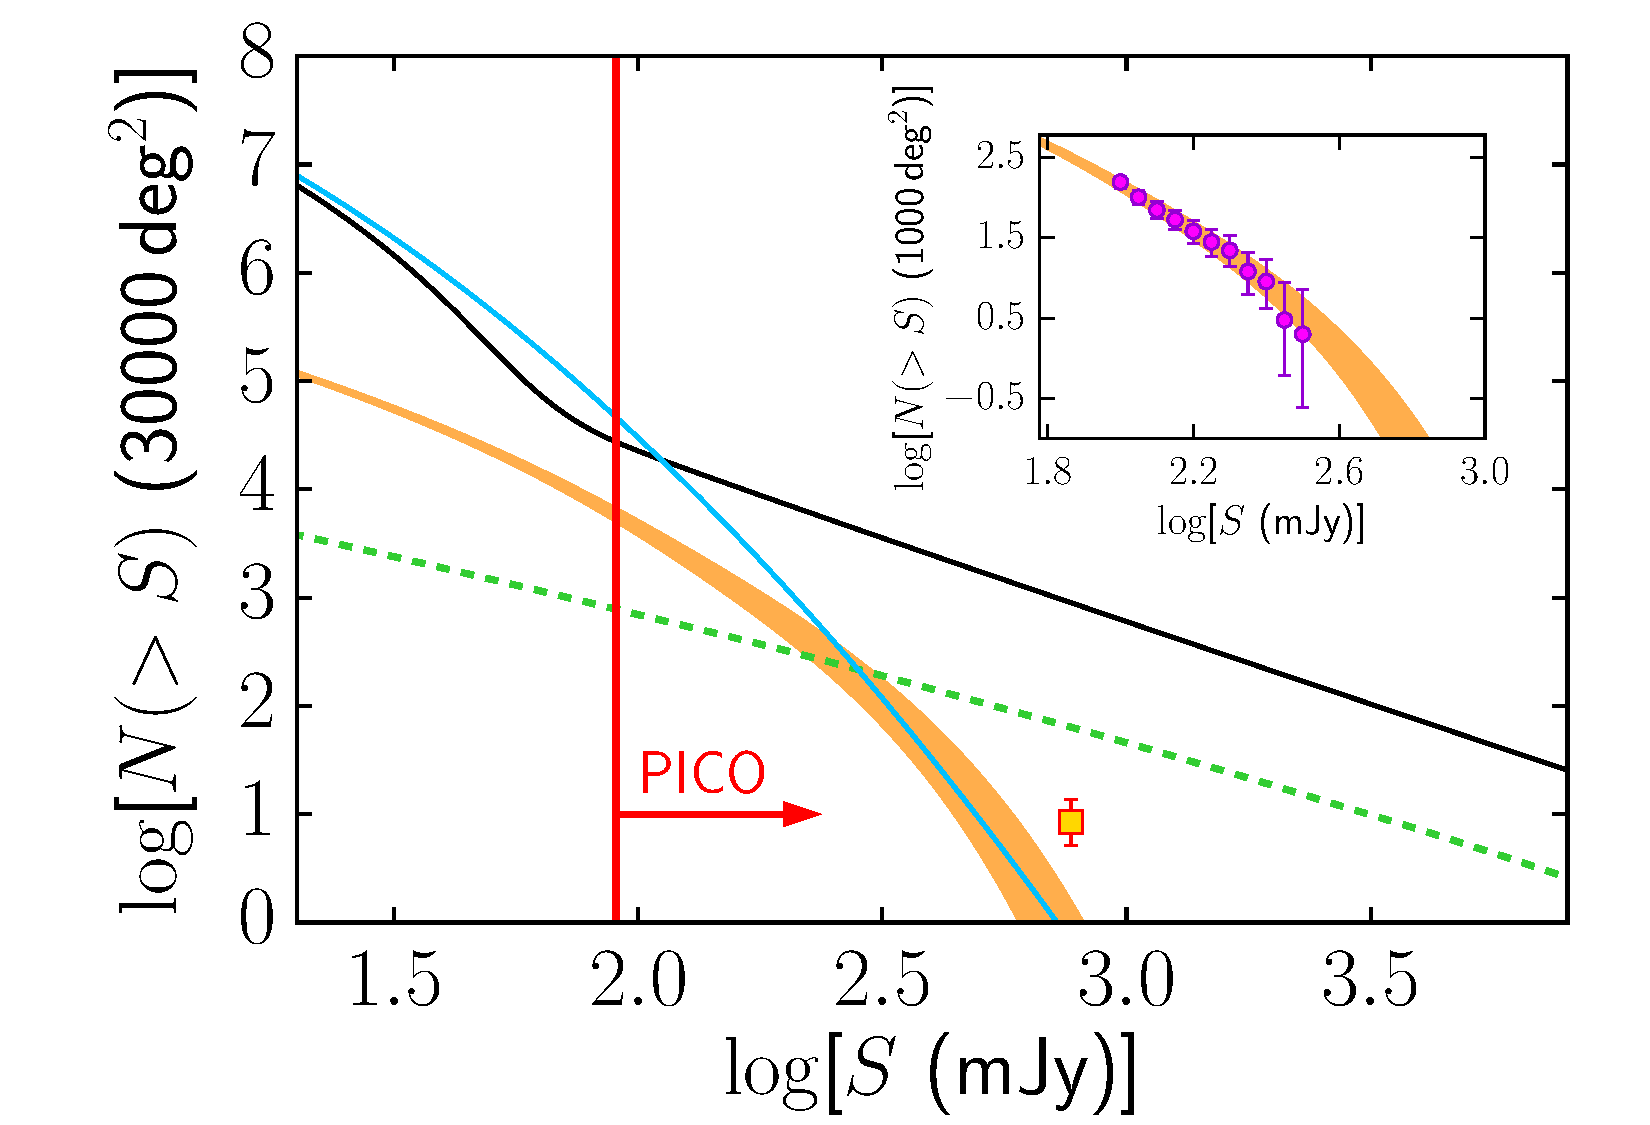
\includegraphics[width=0.4\columnwidth, trim={0 0 0 0cm}, clip]{images/NgtF_pico_NEW.pdf}
\vskip-0.3cm
\caption{ \captiontext
PICO will detect thousands of strongly lensed galaxies and proto-clusters. \textbf{Left panel.} Example spectral energy distributions (SEDs) of dusty star-forming galaxies detectable by PICO, compared with PICO's point-source detection limits (black line) and with the \planck\ 90\% completeness limits (red line~\cite{PCCS2}). PICO will detect nearby galaxies, like M61 (magenta), whose SED was scaled down by a factor of ten, and high-$z$ strongly lensed galaxies, like SMM\,J2133-0102 (blue)  at $z=2.3$~\cite{Swinbank2010} and HLSJ$091828.6{+}514223$ (orange) at $z=5.2$~\cite{Combes2012}. The dashed lines are pre-lensing magnification.  \textbf{Right panel.} Integral counts at 600~GHz of unlensed (black) and strongly lensed, high-$z$ (orange) star-forming galaxies based on fits of \textit{Herschel} counts (inset~\citep{Negrello2017lensed}), also shown are predicted radio source counts (green). The PICO detection region (right of vertical red line) will yield a factor of 1000 increase in strongly lensed galaxies relative to \planck~(yellow square), as well as about 
%the counts of unlensed galaxies have an Euclidean slope, indicative of low $z$.
50,000 proto-clusters (blue)~\citep{Negrello2017protocl}.}
\label{fig:SED3}
\end{center}
\vspace{-0.15in}
\end{figure*}

\comred{PICO was designed to respond to requirements posed by the 7 \ac{SO}s listed in Table~\ref{tab:STM}. 
It will deliver these \ac{SO}s using its own data and data that will become available by known, already funded projects. However, with its combination of angular resolution and frequency coverage PICO will also generate a rich catalog of hundreds of thousands of new sources; see Table~\ref{tab:stm2}. This catalog, consisting of proto-clusters, strongly lensed galaxies, and polarized radio and dusty galaxies, will be mined for years. In some cases follow-up observations by other instruments will be required to provide detailed red-shift data with which to extract the full science information. PICO is the only instrument that can provide a full sky catalog that is not biased by spatial selection.  }

\comor{Kathy Romer says: Table 2 - I like the way this is broken down with ?Current knowledge? summaries. But it only talks about Planck. What about ACT, SPT, SO, balloons etc.? Gianfranco: SPT and ACT are already mentioned in connection to strongly lensed galaxies. So far there is not much from them, in the published literature, on source polarization. On proto-clusters there is the recent discovery of one at z=4.3 (Miller et al. 2018). Perhaps we could add that. }

\subsubsection{Early phases of galaxy evolution}

\comor{Kathy Romer: Section 2.3.1 - page 22 - I noted ?why do we care about lensed high-z galaxies? in the margin. So maybe you need to stress the motivation for this section more? Gianfranco: It is already said that strong lensing provides a unique possibility to look into the structure and kinematics of high-z dusty star-forming galaxies, i.e. to get crucial information on how they form and evolve. I don?t know what to say more.}

PICO will have a crucial role in providing answers to major, still open issues in galaxy formation and evolution. What are the main physical mechanisms shaping the properties of galaxies~\citep{SilkMamon2012, SomervilleDave2015}: in situ processes, interactions, mergers, or cold flows  from the intergalactic medium? And how do feedback processes work? To settle these issues we need direct information on the structure and dynamics of high-$z$ galaxies. But these are compact, with typical sizes of 1--2~kpc~\cite{Fujimoto2018}), corresponding to angular sizes of 0.1--0.2~arcsec at $z\simeq 2$--3. Thus they are hardly resolved, even by ALMA or by HST. If they {\it are} resolved, high enough \ac{SNR}s per resolution element are only achieved for the brightest galaxies, which are probably not representative of the general population.

Strong gravitational lensing provides a solution to these problems. PICO will detect thousands of early forming galaxies whose flux densities are boosted by large factors (Fig.~\ref{fig:SED3}, right panel). Since lensing conserves the surface brightness, the effective angular size is stretched on average by a factor of $\mu^{1/2}$, where $\mu$ is the gravitational magnification, thus substantially increasing the resolving power. A spectacular example is ALMA observations of the \planck-discovered, strongly lensed galaxy PLCK\_G244.8\-+54.9 at $z \simeq 3.0$  with $\mu \simeq 30$~\citep{Canameras2017ALMA}. ALMA observations with a $0.1''$ resolution reached an astounding spatial resolution of 60~pc, substantially smaller than the size of Galactic giant molecular clouds. CO spectroscopy of this object, measuring the kinematics of the molecular gas, gave an uncertainty of 40--50~km/s\comor{put this in context?}. In this specific case, there were no clear indications that mergers or cold flows shaped the galaxy, but similar spectroscopy of another strongly lensed galaxy at $z=5.3$ detected a fast (800 km/s) molecular outflow due to feedback. The outflow carries mass at a rate close to the star-formation rate, and can thus remove a large fraction of the gas that would otherwise be available for star formation.  
% Ca\~{n}ameras et al.~\citep{Canameras2017ALMA} have obtained CO spectroscopy for this object, measuring the kinematics of the molecular gas with an uncertainty of 40--50~km/s. This spectral resolution makes possible a direct investigation of massive outflows driven by AGN feedback at high $z$. Using this technique \citet{Spilker2018} detected a fast (800 km/s) molecular outflow due to feedback in a strongly lensed galaxy at $z=5.3$. They found that the outflow carries mass at a rate close to the star formation rate, and can thus remove a large fraction of the gas that would otherwise be available for star formation.

Currently there are reports of just a few other high-$z$ galaxies that are spatially resolved thanks to gravitational lensing, albeit with less extreme magnifications~\citep{Dye2018, Lamarche2018, Sharda2018}. PICO's catalog will be transformative. \textit{Herschel} surveys have demonstrated that, at the PICO detection limit for $\simeq 500\,\mu$m (600\,GHz), about 25\% of all detected extragalactic sources will be strongly lensed; for comparison, at optical/near-IR and radio wavelengths, where intensive searches have been carried out for many years, the yield is only about 0.1\%, that is more than two orders of magnitude lower~\cite{Treu2010}. To add to the extraordinary sub-mm lensing bonanza, the selection of PICO-detected strongly lensed galaxies will be extremely easy because of their peculiar sub-mm colors (Fig.~\ref{fig:SED3}, left panel), resulting in a selection efficiency close to 100\% \citep{Negrello2010}. 

A straightforward extrapolation of the \textit{Herschel} counts to the much larger area covered by PICO shows that its survey will yield 4,500 strongly-lensed galaxies with a redshift distribution peaking at $2\simlt z \simlt 3$~\cite{Negrello2017lensed}, but extending up to $z> 5$ (Fig.~\ref{fig:SED3}, left panel). If objects like the $z=5.2$ strongly lensed galaxy HLSJ091828.6+514223 exist at higher redshifts, they will be detectable by PICO out to $z>10$.

An intensive high spectral and spatial resolution follow-up campaign of such a large sample will be challenging, but also extremely rewarding, since it will enable a giant leap forward in our understanding of the processes driving early galaxy evolution. It will also open up many other exciting prospects, both on the astrophysical and on the cosmological side (see for example~\citet{Treu2010}). The PICO all-sky surveys will select the brightest objects on the sky, maximizing the efficiency of the effort.

\subsubsection{Early phases of cluster evolution}

PICO will open a new window for the investigation of early phases of cluster evolution, when their member galaxies were actively star forming (and dusty), but the hot IGM was not necessarily in place. In this phase, traditional approaches to cluster detection (X-ray and SZ surveys, and searches for galaxy red sequences) work only for the more evolved clusters, which do include hot IGM; indeed these methods have yielded only a handful of confirmed proto-clusters at $z\simgt 1.5$ \cite{Overzier2016}.\footnote{More high-$z$ proto-clusters have been found by targeting the environment of tracers of very massive halos, such as radio-galaxies, QSOs, sub-mm galaxies. These searches are, however, obviously biased.} \planck~has demonstrated the power of low-resolution surveys for the study of large-scale structure~\cite{Planck2016high_z}, but its resolution was too poor to detect individual proto-clusters \cite{Negrello2017protocl}.  Studies of the high-$z$ 2-point correlation function \cite{Chen2016, Negrello2017protocl} and \textit{Herschel} images of the few sub-mm bright protoclusters detected so far, at $z$ of up to 4 \cite{Ivison2013, Wang2016, Oteo2018}, all of which will be detected by PICO, indicate sizes of $\simeq 1'$ for the proto-cluster cores, nicely matching the PICO FWHM at the highest frequencies.

PICO will detect many tens of thousands of proto-clusters as peaks in its sub-mm maps; see Table~\ref{tab:STM2} and the blue line in the right-hand panel of Fig.~\ref{fig:SED3}. The redshift distribution will extend out to $z\sim4.5$. This catalog will be augmented by 150,000 evolved clusters, detected by the SZ effect. This will constitute a breakthrough in the observational validation of the formation history of the most massive dark-matter halos, traced by clusters, a crucial test of models for structure formation. Follow-up observations will characterize the properties of member galaxies, probing galaxy evolution in dense environments and shedding light on the complex physical processes driving it.

\subsubsection{Additional products of PICO surveys}

PICO will yield a complete census of cold dust, available to sustain star formation in the nearby Universe, by detecting tens of thousands of galaxies mostly at $z\simlt 0.1$. With a statistical population, we will investigate the distribution of such dust as a function of galaxy properties, such as morphology, and stellar mass. \comor{is this not available yet? what's unique? why not in the table?}

PICO will increase by orders of magnitude the number of blazars selected at sub-mm wavelengths and will determine the SEDs of many hundreds of them up to 800\,GHz and up to $z> 5$. Blazar searches are the most effective way to sample the most massive black holes at high $z$ because of the Doppler boosting of their flux densities. PICO's surveys of the largely unexplored mm/sub-mm spectral region will also offer the possibility to discover new transient sources or events, such as blazar outbursts~\cite{Metzger2015}.

PICO will make a giant leap forward in the determination of the polarization properties of both radio sources and of dusty galaxies over a frequency range where ground-based surveys are impractical or impossible. Because of its high sensitivity, PICO will detect in polarization both populations over a substantial flux-density range \comor{vague}, determining directly, for the first time at these wavelengths, number counts in polarized flux density and allowing an accurate correction for their contamination of CMB maps. \comor{refer to point sources in 'foregrounds'}

The anisotropy of the \ac{CIB}, produced by dusty star-forming galaxies over a wide redshift range, is an excellent probe of both the history of star formation and the link between galaxies and dark matter across time. The \planck\ collaboration derived values of the star-formation rate out to $z\sim4$~\cite{2014A&A...571A..30P,2014A&A...571A..18P,madau2014}).
PICO's much lower noise and frequency coverage will give an order of magnitude improvement on the statistical errors for
parameters describing the rate of star-formation history~\cite{Wu:2016hej}. \comor{what are the parameters?}
Similar improvement will be achieved in constraining $M_{\mathrm{eff}}$, the galaxy halo mass that is most efficient in producing star-formation activity. PICO's increased sensitivity to Galactic dust polarization will enhance the separation of signals coming from 
the largely unpolarized \ac{CIB} and polarized Galactic dust; an effective separation of signals currently limits making reliable, legacy-quality \ac{CIB} maps.

%For example, a key parameter in
%simulations of the angular power spectrum of the \ac{CIB}
%is $M_{\mathrm{eff}}$, the galaxy halo mass that is most efficient in producing star
%formation activity. Comparing measurements of the power spectrum to simulations
%constrains this parameter, which informs structure formation models. Current models and measurements
%find $M_{\mathrm{eff}}\sim 10^{12}$ solar masses with about $\mathrm{10\%}$ uncertainty.
%The CMB Probe will constrain this parameter at the percent level.

%Dusty star-forming galaxies trace the underlying dark matter
%field in a broad redshift range. Therefore, a wealth of information will be extracted by
%correlating the anisotropy in the \ac{CIB}
%with multiple dark matter tracers including catalogs of galaxies and quasars,
%and maps of the $\gamma$-ray and the X-ray background~\cite{serra2014,wang2015,cooray2016}.
%These cross-correlations will provide an additional probe of the star formation history, and they will shed light on the interaction between
%light and matter in a broad wavelength range. \comred{the paragraph starts with dark matter, but ends
%with SFR ..?}


\end{document}

%%%%%%%%%%%%%%%%%%%%%%%%%%%%%%%
